% DYSLEXIA SWITCH
\newif\ifdys
		
				% ENABLE or DISABLE font change
				% use XeLaTeX if true
				\dystrue
				\dysfalse


\ifdys

\documentclass[a4paper, 14pt]{extarticle}
\usepackage{amsmath,amsfonts,amsthm,amssymb,mathtools}

\tracinglostchars=3 % Report an error if a font does not have a symbol.
\usepackage{fontspec}
\usepackage{unicode-math}
\defaultfontfeatures{ Ligatures=TeX,
                      Scale=MatchUppercase }

\setmainfont{OpenDyslexic}[Scale=1.0]
\setmathfont{Fira Math} % Or maybe try KPMath-Sans?
\setmathfont{OpenDyslexic Italic}[range=it/{Latin,latin}]
\setmathfont{OpenDyslexic}[range=up/{Latin,latin,num}]

\else

\documentclass[a4paper, 12pt]{extarticle}

\usepackage[utf8x]{inputenc}
\usepackage{lmodern,textcomp}
\usepackage{amsmath,amsfonts,amsthm,amssymb,mathtools}

\fi


\usepackage[french]{babel}
\usepackage[
a4paper,
margin=2cm,
nomarginpar,% We don't want any margin paragraphs
]{geometry}
\usepackage{icomma}

\usepackage{fancyhdr}
\usepackage{array}

\usepackage{multicol, enumerate}
\newcolumntype{P}[1]{>{\centering\arraybackslash}p{#1}}


\usepackage{stackengine}
\newcommand\xrowht[2][0]{\addstackgap[.5\dimexpr#2\relax]{\vphantom{#1}}}

% theorems

\theoremstyle{plain}
\newtheorem{theorem}{Th\'eor\`eme}
\newtheorem*{theorem*}{Th\'eor\`eme}
\newtheorem*{sol}{Solution}
\theoremstyle{definition}
\newtheorem{ex}{Exercice}

% corps
\newcommand{\C}{\mathcal{C}}
\newcommand{\R}{\mathbb{R}}
\newcommand{\Rnn}{\mathbb{R}^{2n}}
\newcommand{\Z}{\mathbb{Z}}
\newcommand{\N}{\mathbb{N}}
\newcommand{\Q}{\mathbb{Q}}

% domain
\newcommand{\D}{\mathcal{D}}


% date
\usepackage{advdate}
\AdvanceDate[0]


% plots
\usepackage{pgfplots}

% for calligraphic C
\usepackage{calrsfs}

%degrees
\usepackage{gensymb}

% SOLUTION SWITCH
\newif\ifsolutions
				\solutionstrue
				\solutionsfalse

\ifsolutions
	\newcommand{\exe}[2]{
		\begin{ex} #1  \end{ex}
		\begin{sol} #2 \end{sol}
	}
\else
	\newcommand{\exe}[2]{
		\begin{ex} #1  \end{ex}
	}
	
\fi

\begin{document}
\pagestyle{fancy}
\fancyhead[L]{Seconde 13}
\fancyhead[C]{\textbf{Trigonométrie \ifsolutions -- Solutions  \fi}}
\fancyhead[R]{\today}

\exe{
	Calculer $\cos(45\degree)$ et $\sin(45\degree)$ de façon \textbf{exacte} à l'aide de l'identité
		\[ \cos^2(\alpha) + \sin^2(\alpha) = 1. \]
}{}

\exe{[14,15 page 141] \, \vspace{-15pt}

	\begin{multicols}{2}
	\begin{center}
	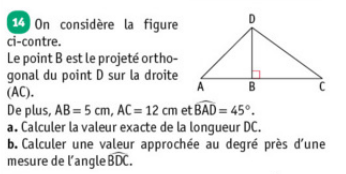
\includegraphics[scale=.75]{14p141.png}
	\, \,
	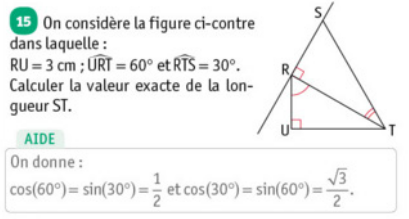
\includegraphics[scale=.6]{15p141.png}
	\end{center}
	\end{multicols}
}{}

\exe{
	En construisant un triangle équilatéral de côté 1, calculer les valeurs suivantes.
		\begin{multicols}{2}
		\begin{enumerate}
			\item $\cos(60\degree)$
			\item $\sin(30\degree)$
			\item $\sin(60\degree)$
			\item $\cos(30\degree)$
			\item $\tan(30\degree)$
			\item $\tan(60\degree)$
		\end{enumerate}
		\end{multicols}
}{}

\exe{
	En étant donné que 
		\begin{align*}
			\sin(15\degree) = \dfrac{\sqrt{6}-\sqrt{2}}4 && \text{ et } && \cos(36\degree) = \dfrac{1+\sqrt{5}}4,
		\end{align*}
	vérifier que $\cos(15\degree) = \dfrac{\sqrt{6}+\sqrt{2}}4$ et donner la valeur \textbf{exacte} de $\sin(36\degree)$.
}{}

%\exe{
%	Sur un terrain, un footballer se trouve à $16,50$ mètres de la ligne de but et à $25$ mètres du poteau de but le plus proche. La largeur des cages est de $7,32$ mètres.
%	
%	Déterminer l'angle de tir $\theta$ en arrondissant au degré près.
%}
%{}

\exe{[Formule de l'aire]
	\begin{multicols}{2}
	Soit un triangle $ABC$ quelconque représenté ci-contre. On pose $a=a_1 + a_2 = BC$.
	
	Monter que
		\[ \text{Aire}(ABC) = \dfrac12 ab \sin(\gamma). \]
	
	\begin{center}
	\begin{tikzpicture}[scale=.8]
		\draw[-, thick, black] (0,0) node{$\bullet$} -- (1.5,0) node[midway, below] {$a_1$};
		\draw[-, thick, black] (1.5,0) -- (4,0) node[midway, below] {$a_2$};
		\draw[-, thick, black] (4, 0) node{$\bullet$} -- (1.5,3) node[midway, right] {$b$};
		\draw[-, thick, black] (1.5,3) node{$\bullet$}-- (0,0) node[midway, left] {$c$};
		
		\node[black, left] at  (0,0) {$B$};
		\node[black, right] at  (4,0) {$C$};
		\node[black, above] at  (1.5,3) {$A$};
		
		\draw[-, thick, black] (1.5,0)-- (1.5,3) node[midway, right] {$h$};
		
		% angle droit
		\draw[-, thick, black] (1.5,.3)-- (1.8,.3);
		\draw[-, thick, black] (1.8,.3)-- (1.8,0);
		
		% angle
		\draw [black,thick,domain=130:180] plot ({4+.5*cos(\x)}, {.5*sin(\x)})
		node[left=5pt, above] {$\gamma$};
	\end{tikzpicture}
	\end{center}
	\end{multicols}
	

}
{}

\exe{[Théorème d'Al-Kashi]
	On souhaite généraliser le théorème de Pythagore aux triangles non nécessairement rectangles.
	Considérons donc le triangle $ABC$ de l'exercice précédent.
	
	\begin{enumerate}
		\item Montrer d'abord que 
			\begin{align*} h = b \sin(\gamma), && \text{ et } && a_2 = b \cos(\gamma). \end{align*}
		\item
		Utilise le théorème de Pythagore pour obtenir
			\begin{align*}
				c^2 &= h^2 + a_1^2, \\
				b^2 &= h^2 + a_2^2. 
			\end{align*}
		\item
		Utiliser $a_1 = a - a_2$ et les expressions obtenues pour conclure que
			\[ c^2 = a^2 + b^2 - 2ab \cos(\gamma). \]
	\end{enumerate}
}
{}


\end{document}
